
To this day, there are many types and variations of ANN, each with its structure and use cases. Here we will briefly introduce the most common ones, such as feed-forward networks, convolutional neural networks, or recurrent neural networks.

\setsecnumdepth{all}
\subsection{Feed-forward Networks}
Feed-forward network (FFN), the first invented ANN and the simplest variation of an ANN. Its name comes from the way how information flows through the network. The data flows in one direction, oriented from the \textit{input layer} to the \textit{output layer}, without cycles. The input layer takes input data, vector $\vec{x}$, producing $\hat{y}$ at the output layer \cite{ffnbrilliant}.

FFN contains several hidden layers of various widths but it can also have no hidden layers at all. By having no back-loops, FFN generally minimizes error, computed by \textit{cost function}, in its prediction by using the \textit{backpropagation} algorithm to update its weight values \cite{mainTypesANN}, \cite{lipton2015critical}.

\begin{figure}[h]
    \centering
    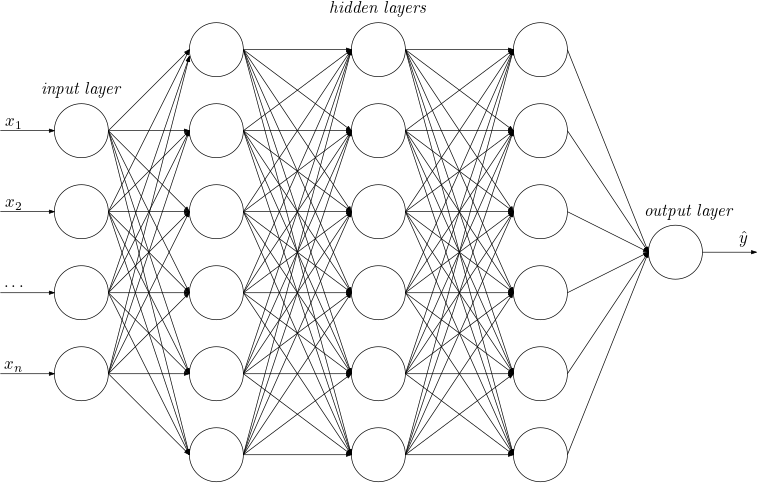
\includegraphics[width=12cm]{ffn.png}
    \caption{Fully connected Feed-forward Neural Network \cite{matous}}
    \label{fig:ffn}
\end{figure}

%=======================================================================================================================

\subsubsection{Cost Function}
Cost function $C(\vec{w})$ is used in ANN's training process. It takes all weights and biases of an ANN as its input, in the form of a vector $\vec{w}$ and calculates a single real number expressing ANN's error in prediction \cite{Goodfellow-et-al-2016}. Higher number expressing poor prediction and as the number gets lower the ANN's output gets closer to the correct result. The main goal of training is to minimize the cost function. 

%=======================================================================================================================
\subsubsection{Backpropagation}
Backpropagation, short of backward propagation of errors, is a widely used algorithm in training FFN using \textit{gradient descent} to find a local minimum of a cost function and update ANN's weights \cite{birlliantbackprop}.

The gradient of a multi-variable function provides us with the direction of the gradient ascent, where we should step to rapidly increase the output and find the local maximum. Conversely, the negative of the gradient points towards the local minimum.'

It is common practice to split training samples into small \textit{batches} of size $n$. For each sample in the batch, we will calculate a gradient descent and use their average gradient descent to update the network's weights. This average gradient descent indicates the adjustments that need to be made to the weights so that the artificial neural network (ANN) moves closer to the correct results \cite{birlliantbackprop}.

\begin{equation}
    {- \gamma \nabla C(\vec{w}_i) + \vec{w}_i \rightarrow \vec{w}_{i+1} }
\end{equation}

$\vec{w_i}$ is weights of the network at the current state (batch), $\vec{w_{i+1}}$ is updated weights, $\gamma$ is the learning rate and $-\nabla C(\vec{w_i})$ is the gradient descent.

%=======================================================================================================================
\subsection{Convolutional Neural Networks}
The primary objective of a Convolutional Neural Network (CNN) is to enable a computer to identify images and objects, making it ideal for image classification and object recognition tasks. 

CNNs are based on the biological processes in the human brain and its connectivity patterns resemble those of the human visual cortex. However, images are perceived differently by the human brain and a computer, with the latter interpreting images as arrays of numbers. As a result, CNNs are designed to work with two-dimensional image arrays, although they can also work with one-dimensional or three-dimensional arrays \cite{mlmastery}.

CNN is a variation of FNN \cite{Goodfellow-et-al-2016}.  It typically consists of an input layer, followed by multiple hidden layers, including several \textit{convolutional layers} and \textit{pooling layers}, and concluding with an output layer.

\setsecnumdepth{all}
\subsubsection{Convolutional Layer}

The convolutional layer's goal is to extract key features from the input image by passing a matrix known as a \textit{kernel} over the input image abstracted into a matrix \cite{mathworkscnn}.

\begin{figure}[h]
	\centering
    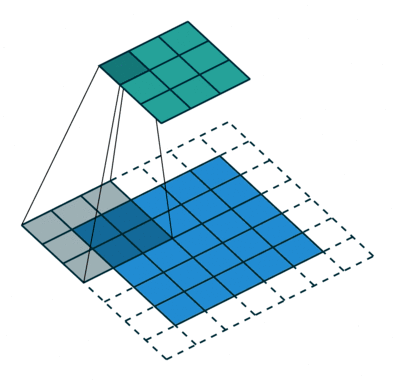
\includegraphics[width=8cm]{conv_layer_padding.png}
	\caption{Convolution of an 5x5x1 image with 3x3x1 kernel \cite{compguideCnn}}
	\label{fig:cnn_conv}
\end{figure}


The outcome of a convolution operation can be either reduced or increased in size. If the size is reduced, it is referred to as \textit{valid padding}. For example, a convolution operation on an 8x8 input image would result in a 6x6 convoluted feature. On the other hand, if the size remains the same or is increased, it is referred to as \textit{same padding} \cite{compguideCnn}.

\subsubsection{Pooling Layer}


Like the convolutional layer, the pooling layer reduces the size of the convolved feature to reduce computational power needed for data processing. It also extracts dominant features that are invariant to rotation and position, making it beneficial for training the model effectively \cite{compguideCnn}.

There are two types of pooling: max pooling and average pooling. Max pooling returns the maximum value from the portion of the image covered by the kernel, acting as a noise suppressant by removing noisy activations and performing de-noising and dimensionality reduction. Average pooling returns the average of all values in the same portion, reducing dimensions as a noise suppression mechanism. It is worth noting that max pooling performs better \cite{compguideCnn}.

\begin{figure}[h]
	\centering
    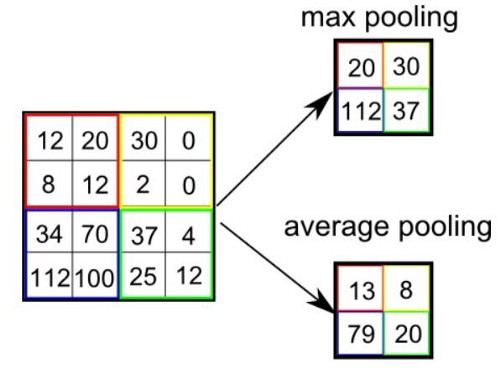
\includegraphics[width=8cm]{conv_pooling.png}
	\caption{Types of pooling \cite{compguideCnn}}
	\label{fig:cnn_pooling}
\end{figure}

%=======================================================================================================================
%\subsection{Recurrent Neural Networks}
%Recurrent Neural Network (RNN) is distinguished by its memory, which can handle input sequences of any length. Its past predictions influence influence the current output. Resulting in different predictions depending on previous inputs in the sequence \cite{rnnDSmedium}.

RNNs are widely used in fields like speech recognition, image captioning, natural language processing, and language translation and are found in popular applications such as Siri, Google Translate, and Google Voice search \cite{ibmrnn}.

To illustrate how RNNs use previous inputs, consider the idiom "feeling under the weather." To understand the meaning, the words must be in a specific order. RNNs take into account the order of the words and use the information from each word to predict the next word in the sequence. Each time step represents a single word, so for example, the third time step represents "the." The hidden state of the RNN holds information from previous inputs, such as "feeling" and "under" \cite{ibmrnn}.

\begin{figure}[h]
    \centering
    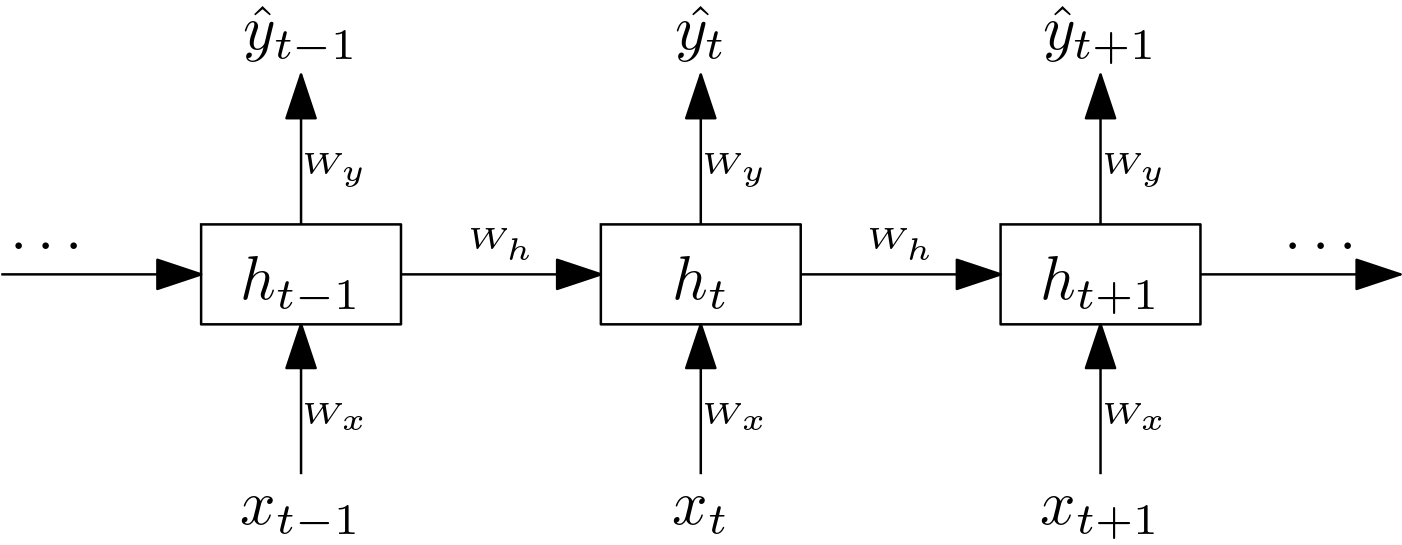
\includegraphics[width=12cm]{rnn_u.png}
    \caption{Unrolled structure of RNN \cite{matous}}
    \label{fig:rnn}
\end{figure}


Figure \ref{fig:rnn} depicts how the RNN network operates at each time step $t$. The current input $\vec{x_t}$ is processed by the network to produce the output $\hat{y}_t$, the next timestep of the input is $x_{t+1}$ with additional input from the previous time step from the hidden state $h_{t}$. This allows the neural network to have a context from previous inputs while processing the current input. The ability to hold past values and work with a context in the data is due to the recurrent units, reffered to as memory \cite{rnnin6}.

The recurrent unit is calculated as follows:

\begin{equation}
    {h_t = f(W_{x}x_t + W_{h}h_{t-1}+\vec{b_h})}
\end{equation}

$f$ is the activation function, $W_x,W_h$ are weight matrixes, $x_t$ is the input, and $\vec{b_h}$ is the vector of bias parameters. The hiddent stat $h_t$ at time step $t=0$ is initialized to $(0,0,...,0)$. The output $\hat{y_t}$ is then calculated as:

\begin{equation}
    {\hat{y}_t = g(W_{y}h_t + \vec{b_y})}
\end{equation}

$g$ is also an activation function, typically softmax, ensuring the output is in the desired class range. $W_y$ is the weight matrix, and $\vec{b_y}$ is a vector of biases determined during the learning process.

Training RNNs uses a modified version of the backpropagation algorithm called \textit{backpropagation through time} (BPTT). This process works by unrolling the RNN \cite{Goodfellow-et-al-2016}, computing the losses across each time step, and then using the backpropagation algorithm to update the weights. More on RNN in \cite{lipton2015critical} by Lipton et al.


%=======================================================================================================================
%\subsection{Long Short-Term Memory}
%Consider a task where we attempt to predict the last word in a sentence "The clouds are in the \textit{sky}". It is fairly obvious the last word is meant to be "\textit{sky}". The gap between the relevant information and the prediction place is small, RNNs can learn to use past information and make accurate predictions. However, if we consider "I grew up in Spain... I speak fluent \textit{Spanish}", the gap between the relevant information and predicting word is large. As the gap grows, RNNs are unable to handle the task. Such problem is called \textit{long-term dependencies} \cite{colahLSTM}.

Long Short Term Memory networks (LSTM), first introduced by Hochreiter S. and Schmidhuber J. \cite{hochreiterLSTM}, are RNN architecture with the ability to handle long-term dependencies. LSTMs replace RNN's hidden states with \textbf{LSTM Cells} and add connections between cells, known as \textit{cell states} or $c_{t}$. Each LSTM Cell consists of three gates that regulate the input and output of the cell and its calculation runs as follows:

1. \textbf{Forget Gate}: Controls which information to keep and which to discard. \textit{Sigmoid function} produces a value ranging from 0 to 1 base on the information from the previous hidden state and from the current input. The value closer to 0 indicates that the information should be discarded, while a value closer to 1 means it should be kept.

\begin{equation}
    {f_t = \sigma(W_{x_f}x_t + W_{h_f}h_{t-1}+\vec{b_f})}
\end{equation}

2. \textbf{Input Gate}: Decides which information should be updated. The sigmoid function a value between 0 and 1 based on the previous hidden state and the current input state. A value close to 0 indicates unimportant information, while a value close to 1 indicates important information.

\begin{equation}
    {i_t = \sigma(W_{x_i}x_t + W_{h_i}h_{t-1}+\vec{b_i})}
\end{equation}

The information from the previous hidden state and the current input state are processed by a \textit{tanh} function, which results in values ranging from -1 to 1.

\begin{equation}
    {g_t = \tanh(W_{x_g}x_t + W_{h_g}h_{t-1}+\vec{b_g})}
\end{equation}

The decision on how to update the cell is obtained by multiplying sigmoid output and $\tanh$ output. With all the required values available, we can now calculate the \textit{cell state} as follows:

\begin{equation}
    {c_t = i_t \odot g_t + f_t \odot c_{t-1}}
\end{equation}


3. \textbf{Output Gate}: Determines what information should the next hidden state contain. The previous hidden state and the current input are passed into a sigmoid function.

\begin{equation}
    {o_t = \sigma(W_{x_o}x_t + W_{h_o}h_{t-1}+\vec{b_o})}
\end{equation}

Passing the newly modified cell state into a tanh function and multiplying its output with the sigmoid output, we get the hidden state \cite{guideLSTM}.

\begin{equation}
    {h_t = o_t \odot tanh(c_t)}
\end{equation}


The output $\hat{y}_t$ is calculated the same way as regular RNN \cite{matous}.

\begin{equation}
    {\hat{y}_t = g(W_{y}h_t + \vec{b_y})}
\end{equation}

\begin{figure}[h]
    \centering
    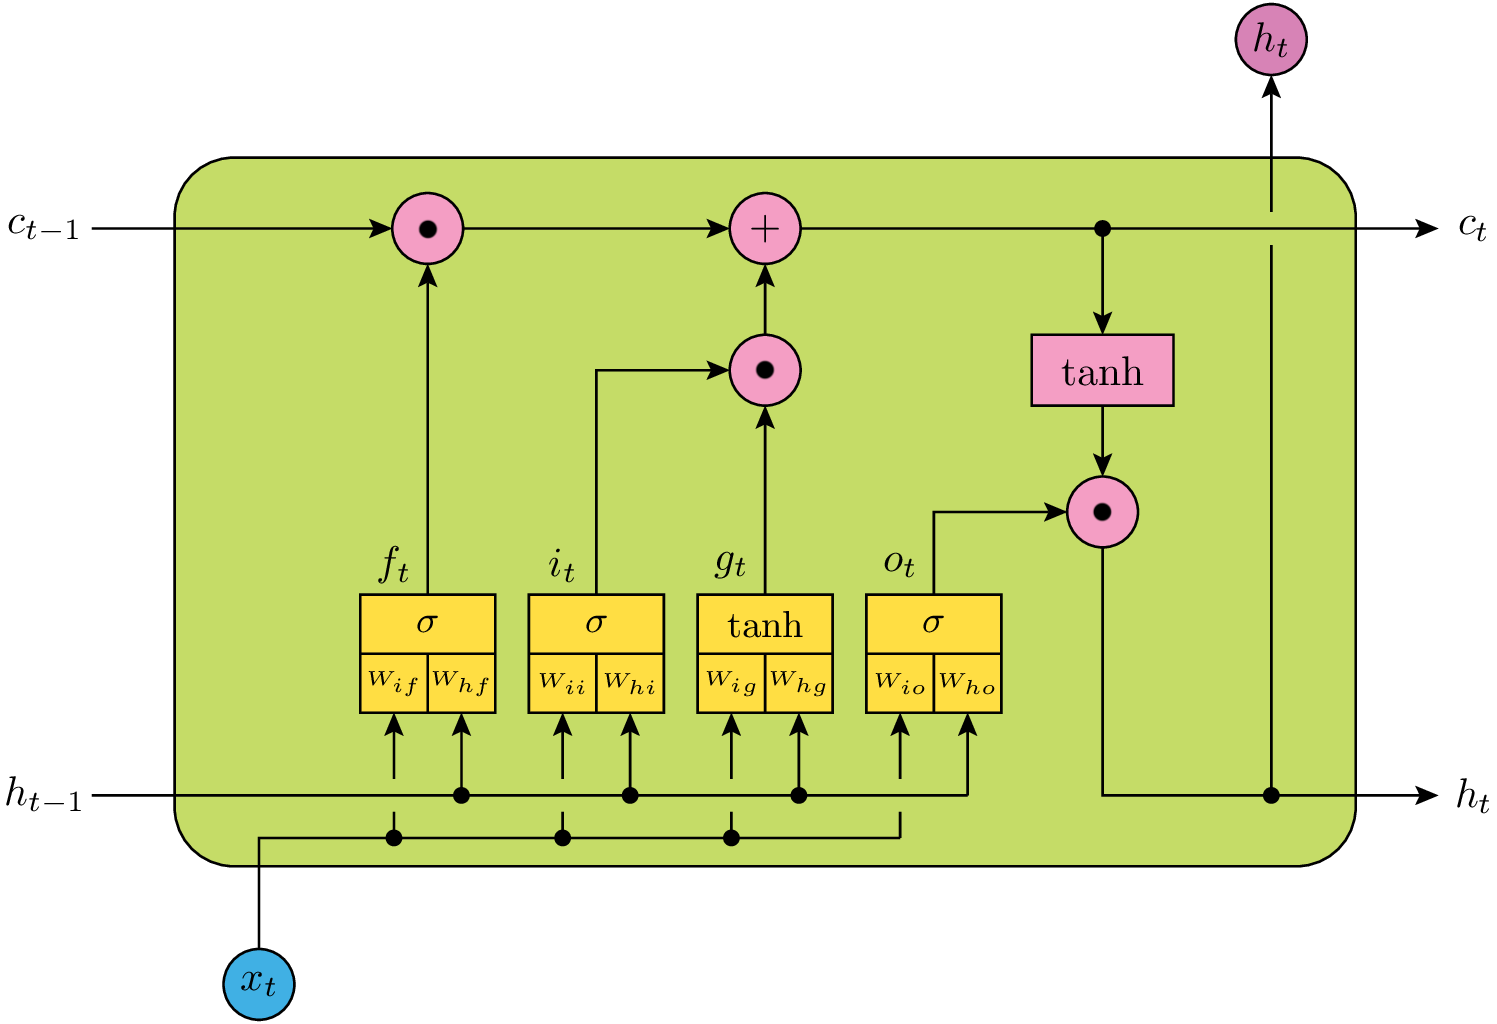
\includegraphics[width=10cm]{lstm_cell.png}
    \caption{LSTM cell \cite{lstmcell_img}}
    \label{fig:lstmCell}
\end{figure}
%=======================================================================================================================
\subsection{Graph Neural Networks}
Graphs are commonly used to describe and analyze entities with relations or interactions. Still, today's deep learning modern toolbox is specialized for simple data types, e.g., grids for images, sequences for text or speech. These data structures have spatial locality, the grid size or sequence length is fixed and can be resized. We can also determine the starting position and ending position. Graph problems are, on the other hand, much more challenging to process as they have arbitrary size and complex topological structure (i.e., no spatial locality like grids). Graphs also have no fixed node ordering or reference point compared to grids or sequences. For such Franco Scarselli et al. introduced graph neural network (GNN) \cite{graph}.

GNN is designed similarly to CNN. As previously noted, CNN operates on images. Given an image, a rectangular grid, the convolutional layer takes a subpart of the image, applies a function to it, and produces a new part, a new pixel. This is iterated for the whole image. What actually happened is the new pixel resulted in aggregated information from neighbors and itself. This cannot be easily applied to graphs as they have no spatial locality and no fixed node ordering. As implied, a GNN design stands on passing and aggregating information from neighbors. 

\subsubsection{Node embedding}

Graphs require a concept called node embedding. The general idea is to map nodes to a lower dimensional embedding space, where similar nodes in the embedding space approximate similarity in the graph network. For example, we can map a 3D vector to a 2D vector. Node embedding is useful for learning node representations and similarities and can be trained on graphs with arbitrary structures.

Nodes have embeddings at each layer. Taken node $v$, its layer-0 embedding would be its feature vector $x_v$. If we want layer-1 embedding, we will explore node $v$'s neighbors. These neighbors are so-called one hop away from our original vector $v$. We take the feature vector of these nodes and aggregate the information into one single $x_v$ feature vector. Layer-k would get information from nodes that are k hops away. 

\begin{figure}[h]
  \centering
  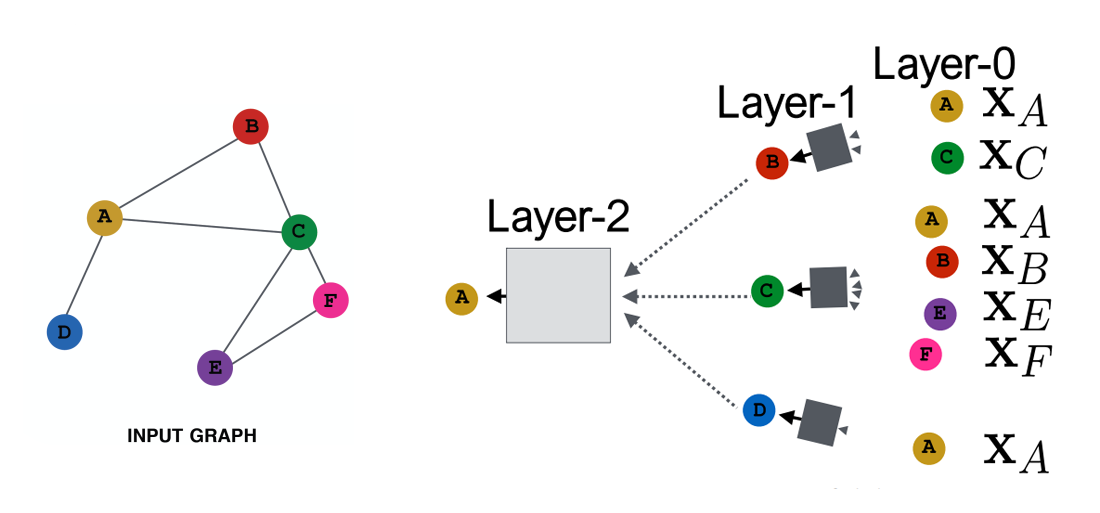
\includegraphics[width=12cm]{gnn_layers.png}
  \caption{Layer-2 embedding applied on node $A$ aggregating infromation from its neighborhood \cite{stanford}}
  \label{fig:gnn_layers}
\end{figure}

The described process is called neighborhood aggregation. If we want to predict node $v$, we need information from its neighborhood, meaning we need a way to propagate the message. Messages are passed and transformed through edges. All received messages are aggregated into a new message and then passed on. This is done systematically for every node in the graph.

The aggregation itself is done by a neural network. This implies the key difference from a typical ANN. Every node gets to define its own neural network and GNN is defined by multiple neural networks.

\begin{figure}[h]
  \centering
  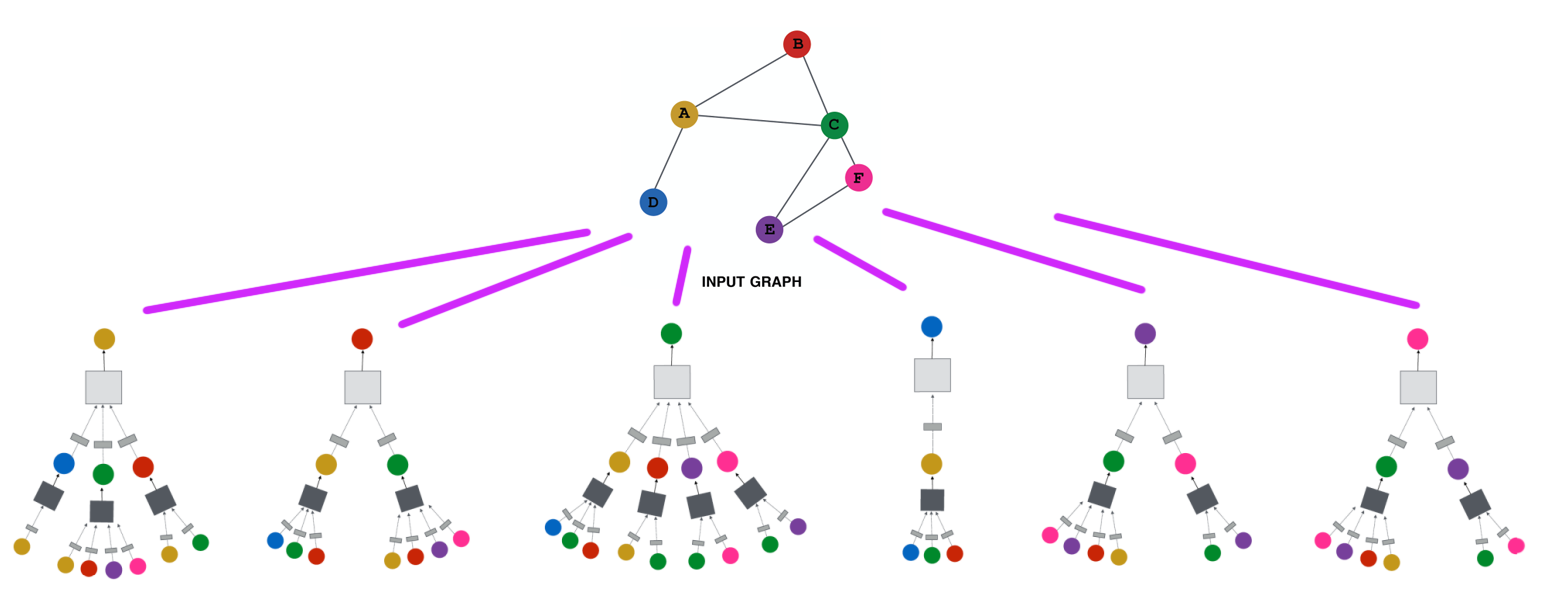
\includegraphics[width=12cm]{gnn_graph.png}
  \caption{Neural network of each node for given input node graph \cite{stanford}}
  \label{fig:gnn_graph}
\end{figure}

Using a neural network for each node in the graph, we generate a low-dimensional vector representation, embedding. The network optimizes its parameters to capture important information about the node graphs. The optimization is typically done by minimizing a loss function expressing dissimilarity between predicted and targeted node embeddings. Similar nodes are close to each other, whereas dissimilar are embedded far apart. 

\subsubsection{Geometric graphs}
TODO SECTION
Geometric graph is a graph where its nodes represent coordinates in d-dimensional space. Invariant to translation, rotation and scale

... todo more mat... 

%=======================================================================================================================